\chapter{Results}

This section will summarize the results that the described algorithm achieved on the described datasets. Before going into detail about the performance on the SIDDATA-dataset (\ref{sec:dataset_siddata}), a brief summary of the results on the placetypes-dataset (\ref{sec:dataset_placetypes}) should demonstrate if the specific implementation can achieve comparable results to \mainalgos, thus putting the other results into perspective in terms of what the algorithm can realistically achieve on dedicated high-quality datasets.

\section{How to Evaluate}

Due to the implemented algorithm being an \gls{unsupervised} algorithm, there is no explicit target value for each of the considered samples, making it impossible to straight-forwardly apply well-known \gls{ml} metrics such as \Gls{acc} or \gls{f1}. What this algorithm tries to achieve is a lot \textit{fuzzier} than in the realm of classification: The end-goal of it is to embed the given \glspl{entity} into a vector-space that consists of semantically meaniningful directions, so the only actual metric would be a comparison checking if the respective categorization here corresponds closely to human judgement. To do that, the best evaluation is likely a study that asks for feedback of users that see the results of a developed system\footnote{An example for such a system is the \textit{Movie Tuner} interface from \textcite{VISR12}, reprinted as \autoref{fig:movetuner}.}. \textcite{Derrac2015} performed crowdsourcing experiments on CrowdFlower\footnote{\url{http://www.crowdflower.com}}, asking users among other tasks which of several candidates could best describe the difference between two movies. They also compared their results with those of running the supervised algorithm of \cite{VISR12} on a subset of their data. Furthermore they tested if the explainable classifiers generated from this algorithm (see \autoref{sec:reasoning}) \q{help users spot incorrect classifications} \cite[48]{Derrac2015}, as well as if their algorithmic classification corresponds to human judgement\footnote{The task was set only for classification into OpenCYC and Foursquare Taxonomies of the placetypes-dataset (see column `\textbf{classification classes}' in \autoref{tab:all_datasets}).}. 
\todoparagraph{TODO: Should I also quickly mention their results?}
While similar studies could be done in the SIDDATA-\gls{dsa} \cite{Schurz2021} without additional costs, carrying these out is outside the scope of this thesis.

This thesis relies on both qualitative analysis and quantitative anlaysis in order to quantify the algorithm's performance.\\ 
In the \textit{qualitative analysis}, exemplary partial results of the algorithm will be showcased that should intuitively show if what the algorithm does looks \textit{realistic} from a human perspective. It should be noted that analyses of this kind are always to be taken with care, because there is no guarantee that the picked examples are actually representative and not the result of (intentional or accidental) cherry-picking.\footnote{\todoparagraph{TODO: and I'll also quickly show that DESC15 weren't always perfect as well}}\\
To also generate unambiguous facts, a \textit{quantitative analysis} was performed as well. Due to the aforementioned lack of obvious metrics however, workarounds must be found to generate clear quantifiable performance estimates. Like \mainalgos, this thesis makes use of \textit{Shallow Decision Trees} that are trained to recover a known category of the dataset from the generated semantic directions.
% TODO: *HOW* I evaluated is not part of the results, is it?!

\includeMD{pandoc_generated_latex/4_0_results}

The plots \ref{fig:scatter_mds_movies} and \ref{fig:scatter_mds_placetypes} show a 2D-representation of the MDS %TODO: link MDS anyway, if not to the glossary than to the section
of the movies- and placetypes-dataset as made public by \textcite{Derrac2015}\footnote{\url{https://www.cs.cf.ac.uk/semanticspaces/}}. Visually comparing them to their equivalent to the SIDDATA-dataset (\autoref{fig:scatter_mds}) \todoparagraph{shows that while the movie-embeddings looks pretty clustered}, the clustering of the placetypes-dataset looks in fact a lot worse than that of the SIDDATA-dataset.
%TODO: obviously write again. What do we see? A 2D-Version of the MDS. If we see very distinct clusters in that, we can conclude that it sounds possible that we can detect whatever-we-colored-by from this embeddings to an okay degree.

\begingroup
\renewcommand*{\arraystretch}{2}
\begin{table}[]
	\centering
	\begin{tabular}{rccccc}
										  & \multicolumn{3}{c}{\textbf{Feature vectors}}           & \textbf{Candidates} & \textbf{Cluster Elements}   \\
										  & \textbf{Mean L.} & \textbf{Vectors} & \textbf{Clusters} &                     & \textbf{($\kappa\geq0.1$}) \\
    \midrule	
										  
	\textbf{movies \cite{Derrac2015}}     & 12083            & 589727           & 3864              & 22903               & 9389              		   \\
	\textbf{placetypes \cite{Derrac2015}} &                  &                  &                   &                     &                   		   \\
	\textbf{SIDDATA}                      &                  &                  &                   &                     &                  
	\end{tabular}
	\caption{Statistics on generated features of the algorithm}
	\label{tab:generated_stuff}
\end{table}
\endgroup
% movies:
% feature vecs: 38649 keys with 0-33k terms each (sum: 589727 terms) 
% candidate-terms: 22903 (unclustered)
% clusters: ndims*2 -> for 20D: 9389 (-> 9429 words in $T^{0.1}$)}		
% movies: 15.000
% ppmi-weighted feature vectors: 38649 keys with bag-of-words between 0 words and 33k words (but mostly couple 1000s), all in all 589727 unique terms
% candidate-terms: 22903 (unclustered)
% clusters: ndims*2 clusters with all in all (for 20d) 9389 values (->9429 words have kappa>=0.5)

\begin{table}
	\resizebox{0.6\textwidth}{!}{%
	\caption{This algorithm on Placetypes}
	\begin{tabular}{llrrr}
	\toprule
	 & \textbf{Depth:} & \textbf{1} & \textbf{2} & \textbf{3} \\
	\textbf{1vsRest} & \textbf{Balanced} &  &  &  \\
	\midrule
	\multirow[t]{2}{*}{\textbf{False}} & \textbf{False} & 0.427 & 0.474 & 0.477 \\
	 & \textbf{True} & 0.057 & 0.107 & 0.139 \\
	\cline{1-2}
	\multirow[t]{2}{*}{\textbf{True}} & \textbf{False} & {\cellcolor{lightgreen}} 0.745 & {\cellcolor{lightgreen}} 0.795 & {\cellcolor{lightgreen}} 0.811 \\
	 & \textbf{True} & 0.529 & 0.660 & 0.681 \\
	\bottomrule
	\end{tabular}
	}
\end{table}


\section{Qualitative Analysis}

\begin{figure}[h]
	\begin{center}
	  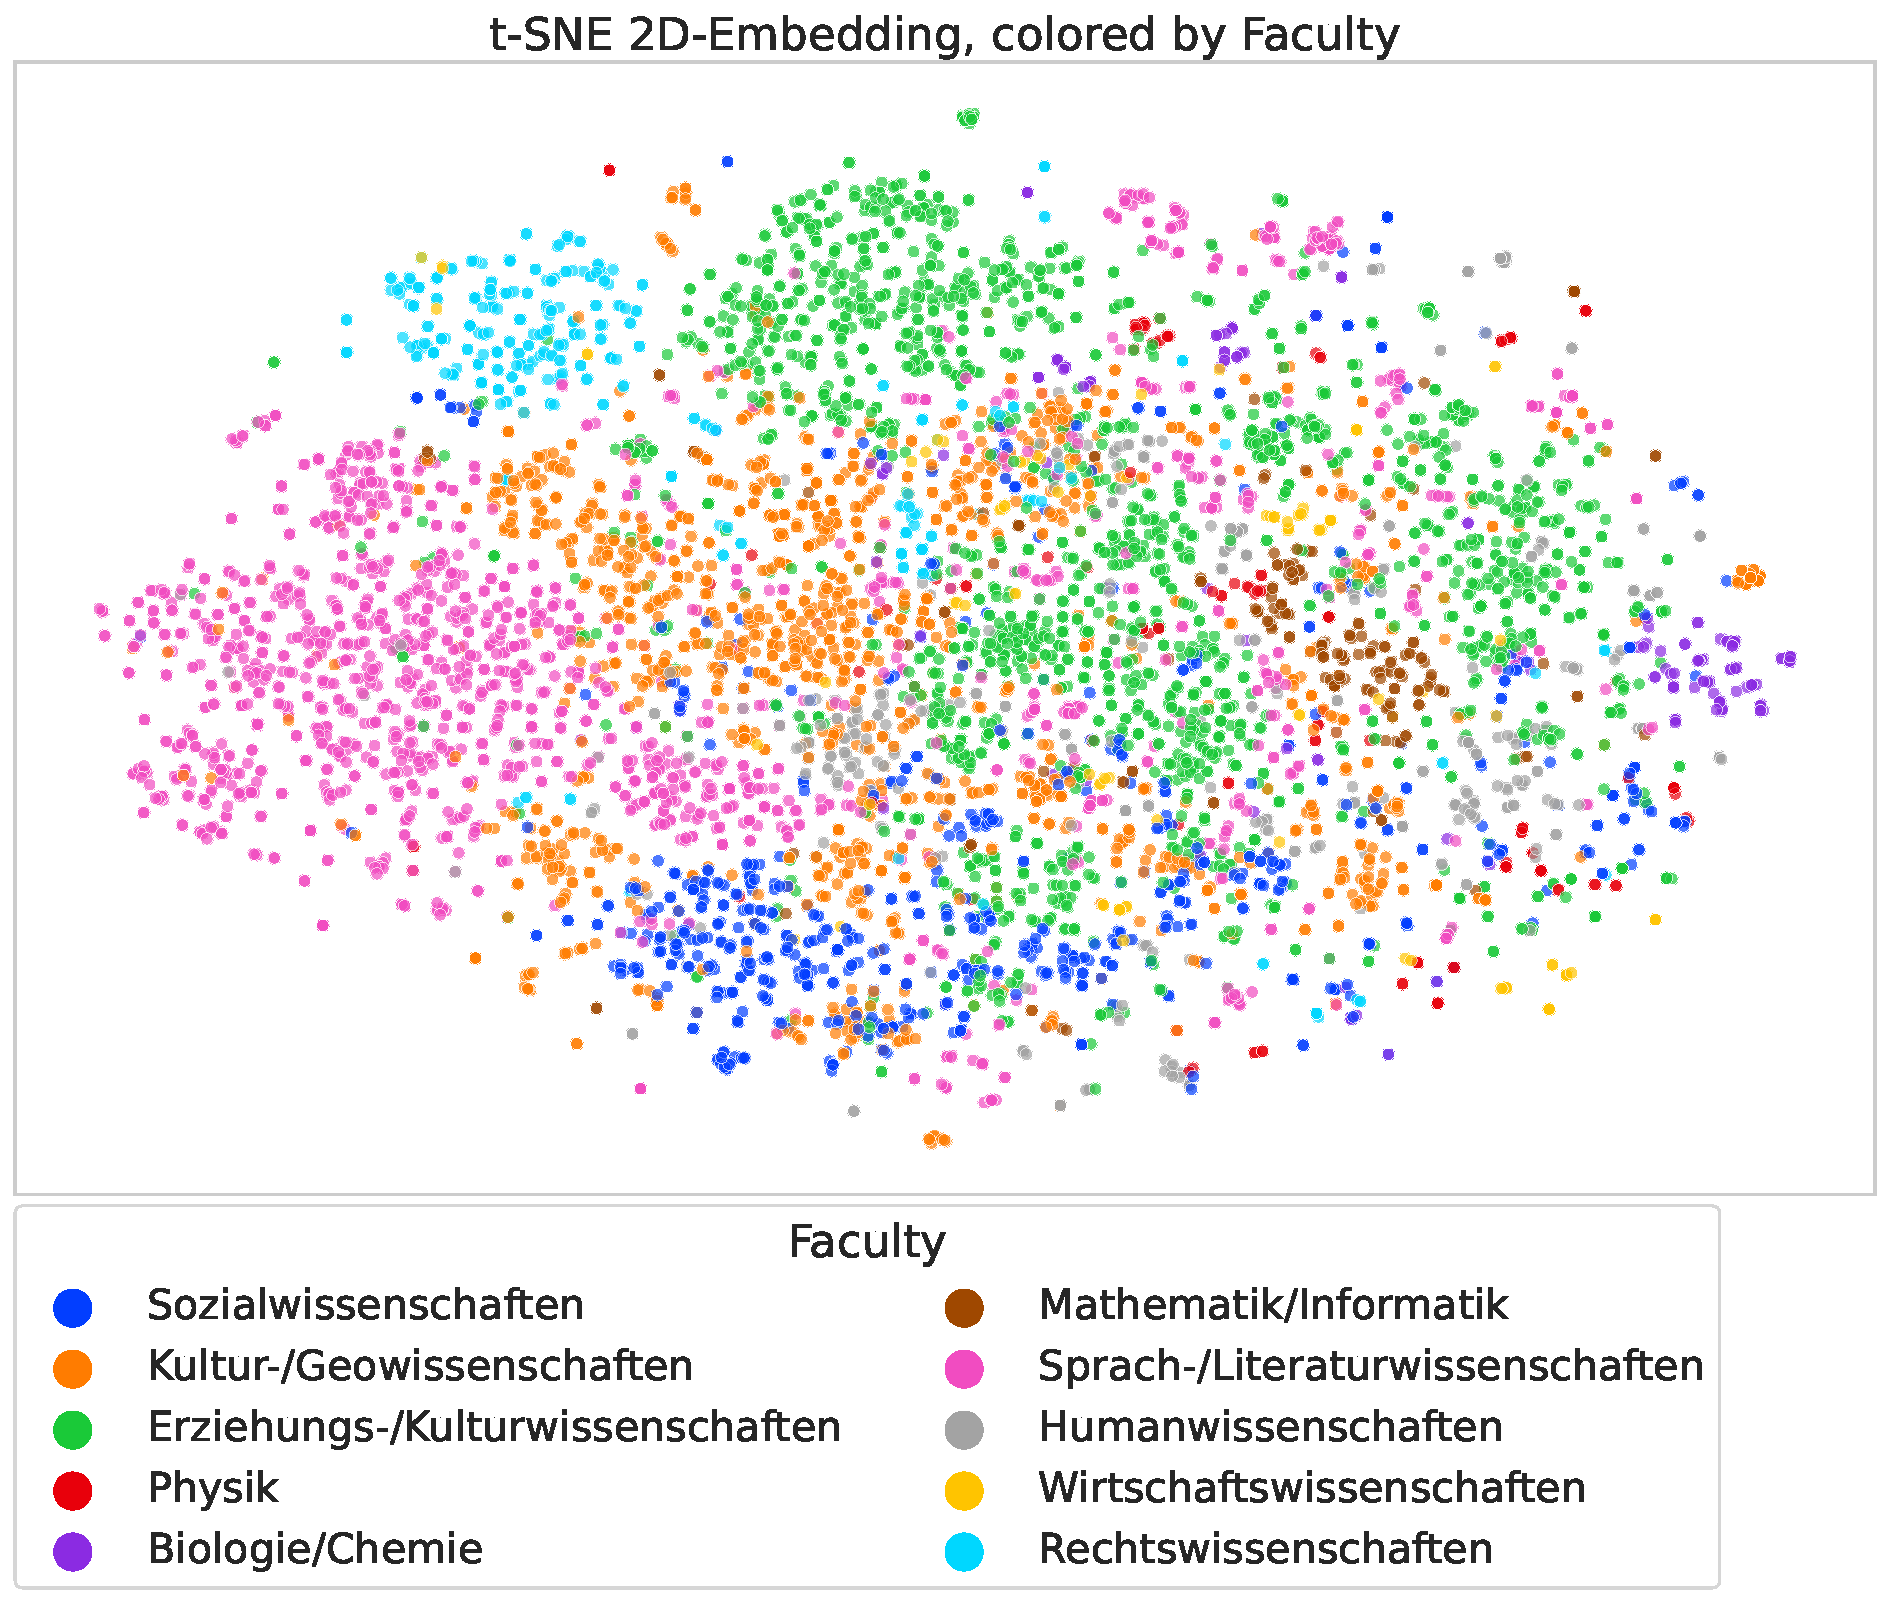
\includegraphics[width=0.9\textwidth]{graphics/dataset_new/scatter_mds_tsne_e2a70a9bf2.pdf}
	  \slcaption{2D Visualization of the Course-Dissimilarity-Matrix, generated with \gls{tsne}. See \url{https://github.com/cstenkamp/derive_conceptualspaces/blob/main/notebooks/text_referenced_plots/visualize_embeddings.ipynb} for the origin of this plot as well as a 3D-plot on unaltered 3D-MDS-data that doesn't rely on t-SNE.}
	  \label{fig:scatter_mds}
	\end{center}
\end{figure}



\begin{figure}[h]
	\begin{center}
	  \makebox[\textwidth][c]{
		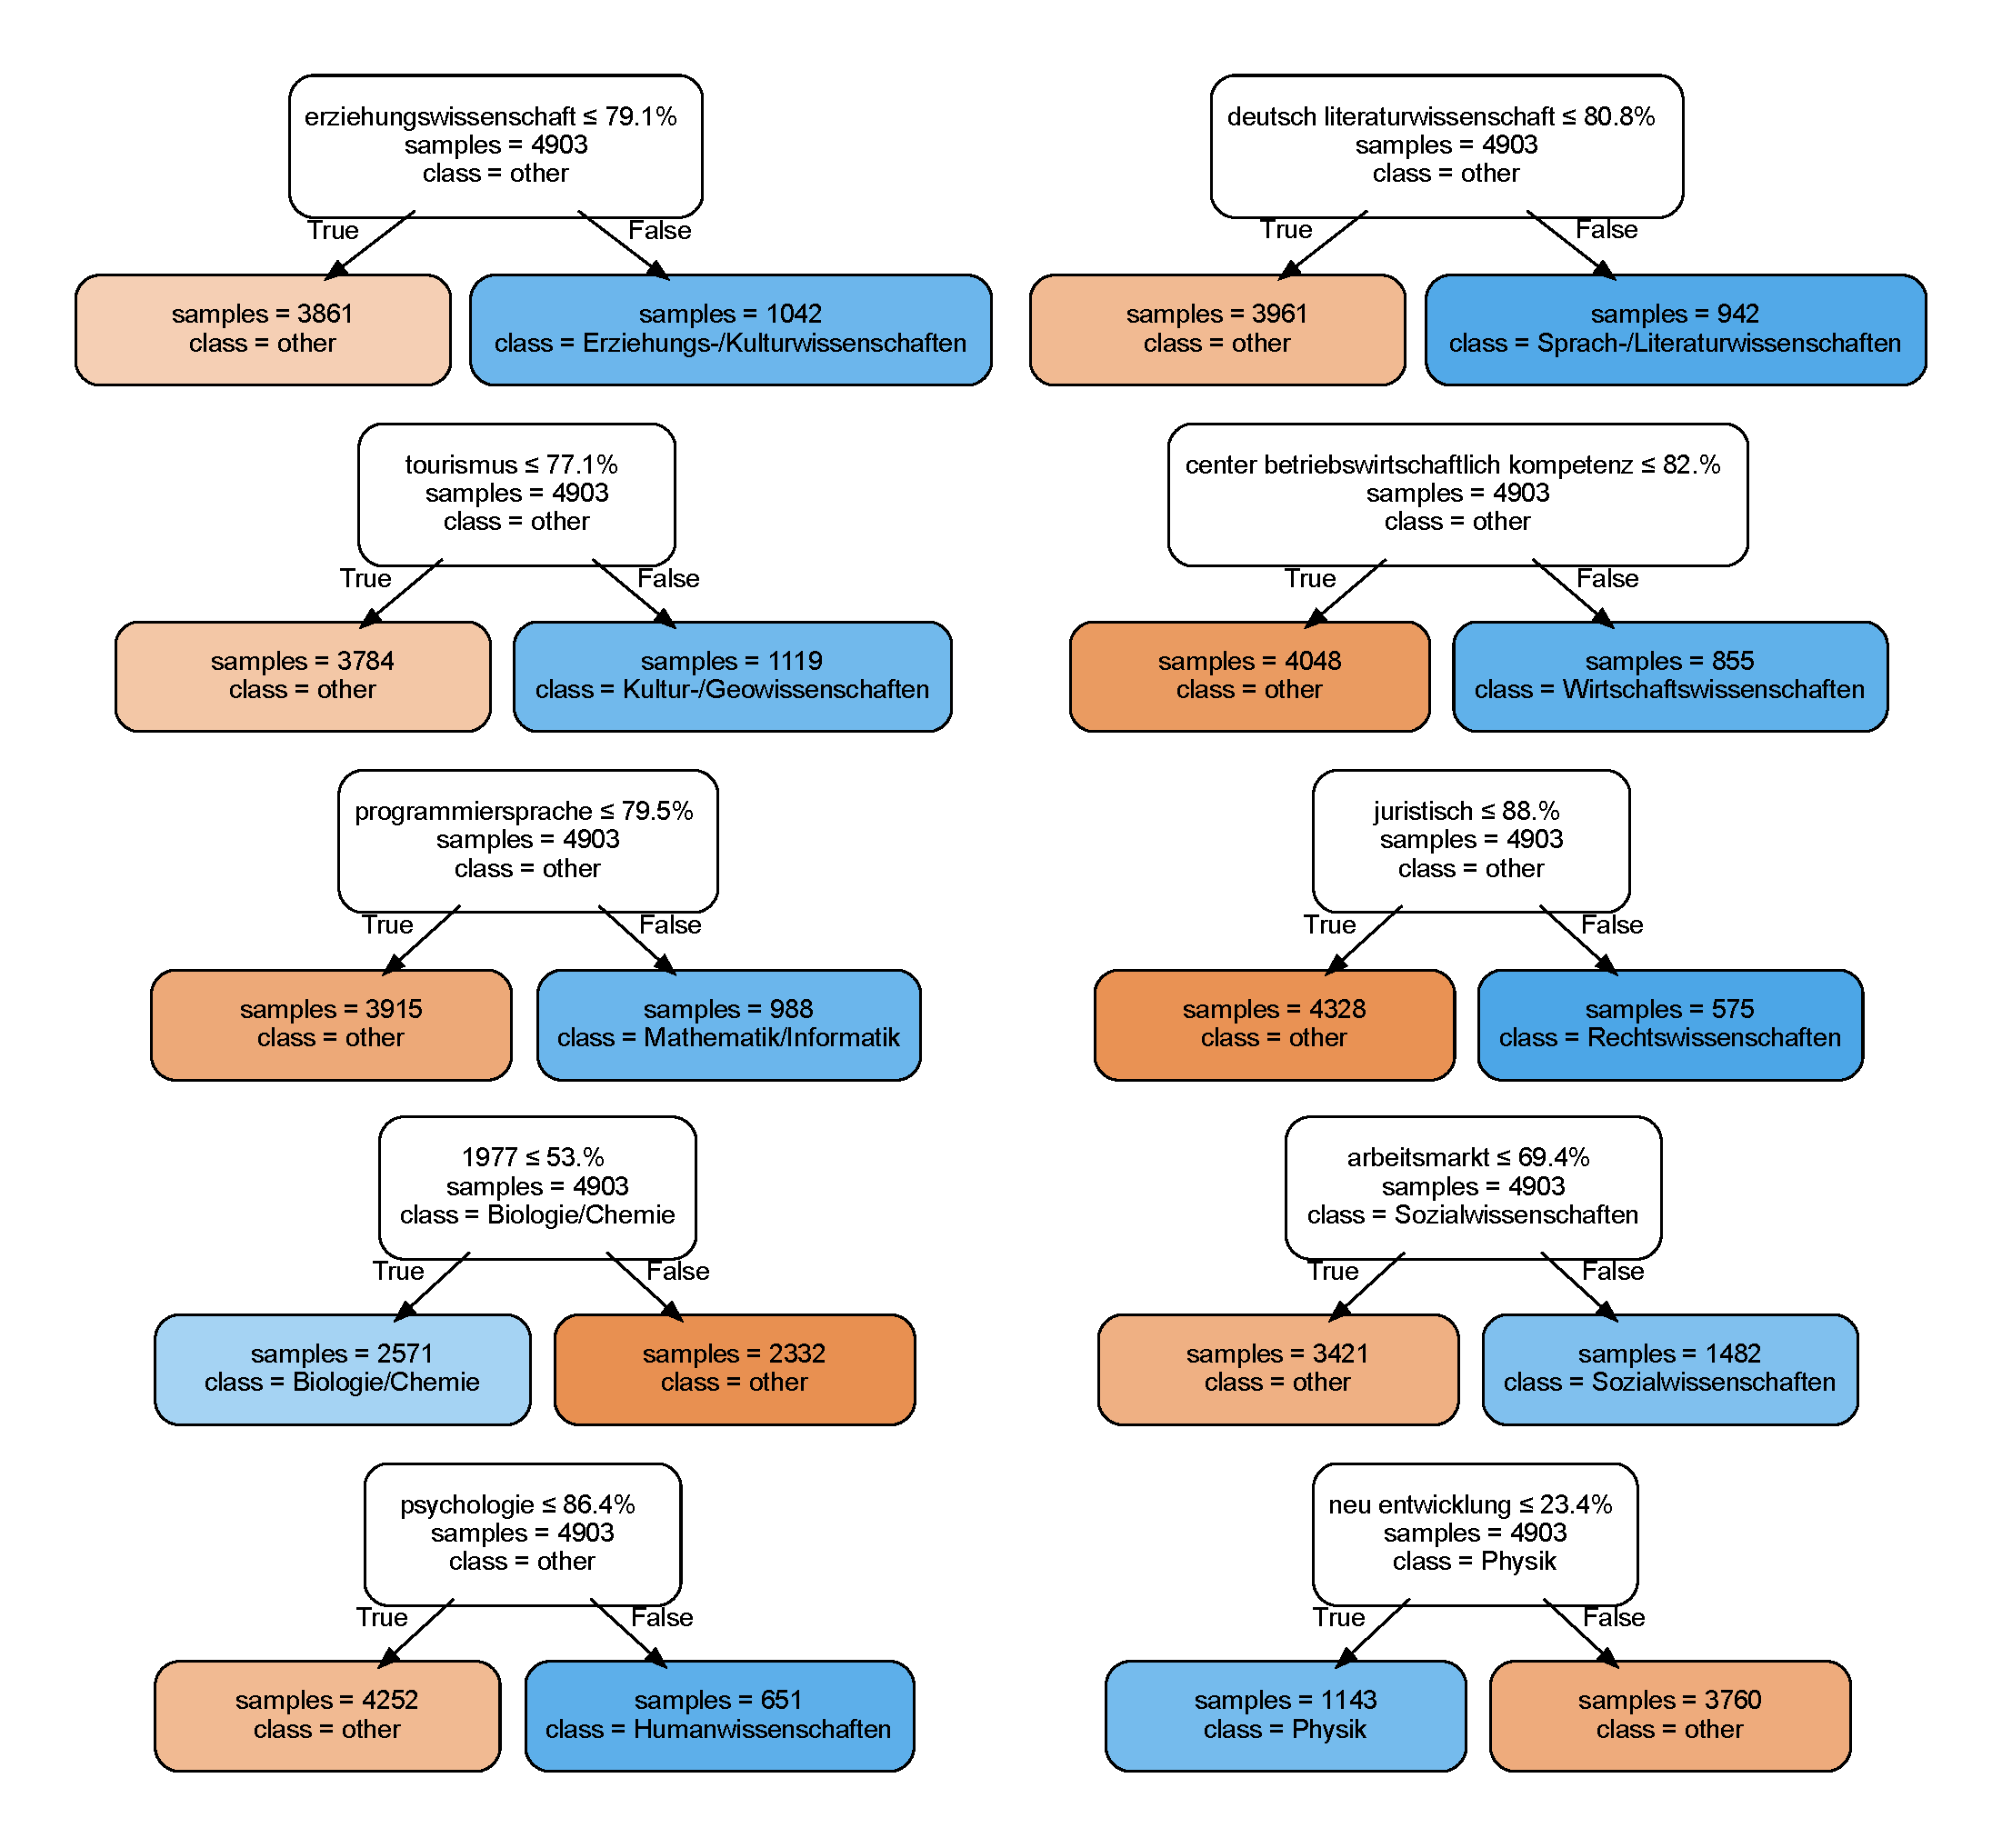
\includegraphics[width=1.3\textwidth]{graphics/dataset_new/dims_for_fb.pdf}
		\slcaption{Learned Level-1-Decisiontrees.}
		\label{fig:dims_for_fb}
	  }
	\end{center}
\end{figure}

\begin{figure}[h]
	\begin{center}
	  \makebox[\textwidth][c]{
		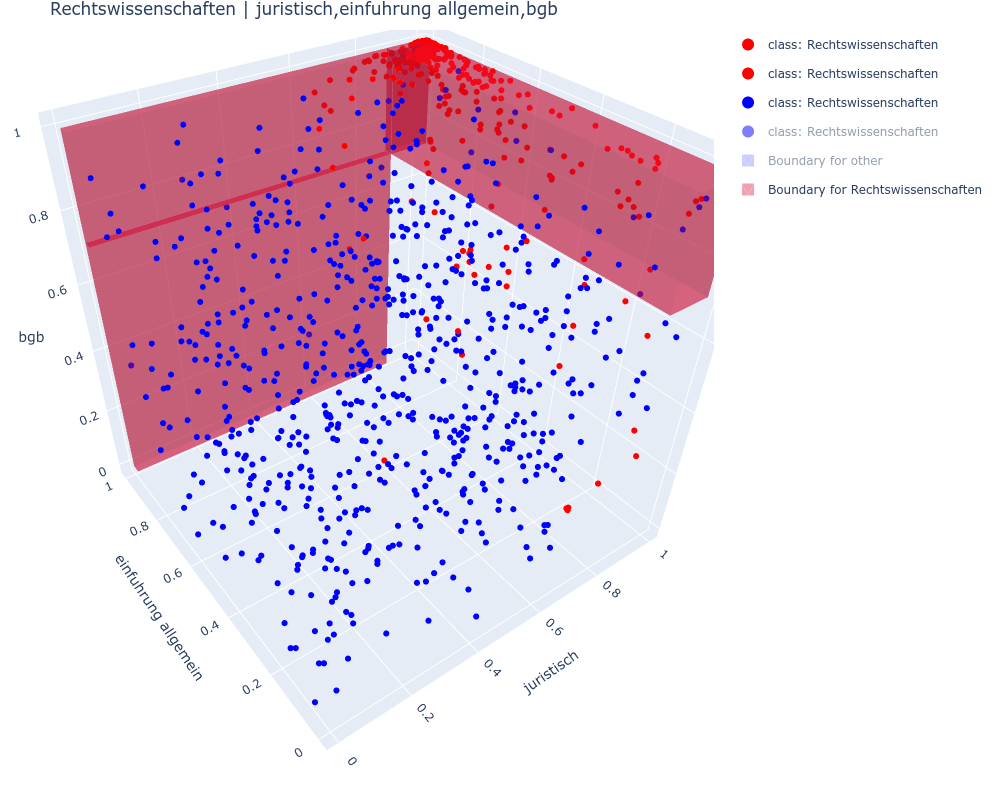
\includegraphics[width=1.1\textwidth]{graphics/dataset_new/boxes_rechtswis.png}
		\slcaption{A classification with a Level-3-Decisiontree. Visualize in 3D: \url{https://github.com/cstenkamp/derive_conceptualspaces/blob/main/notebooks/text_referenced_plots/display_top3_SIDDATA.ipynb} }
		\label{fig:boxes_rechtswis}
	  }
	\end{center}
\end{figure}


\begin{figure}[h]
	\begin{center}
	  \makebox[\textwidth][c]{
		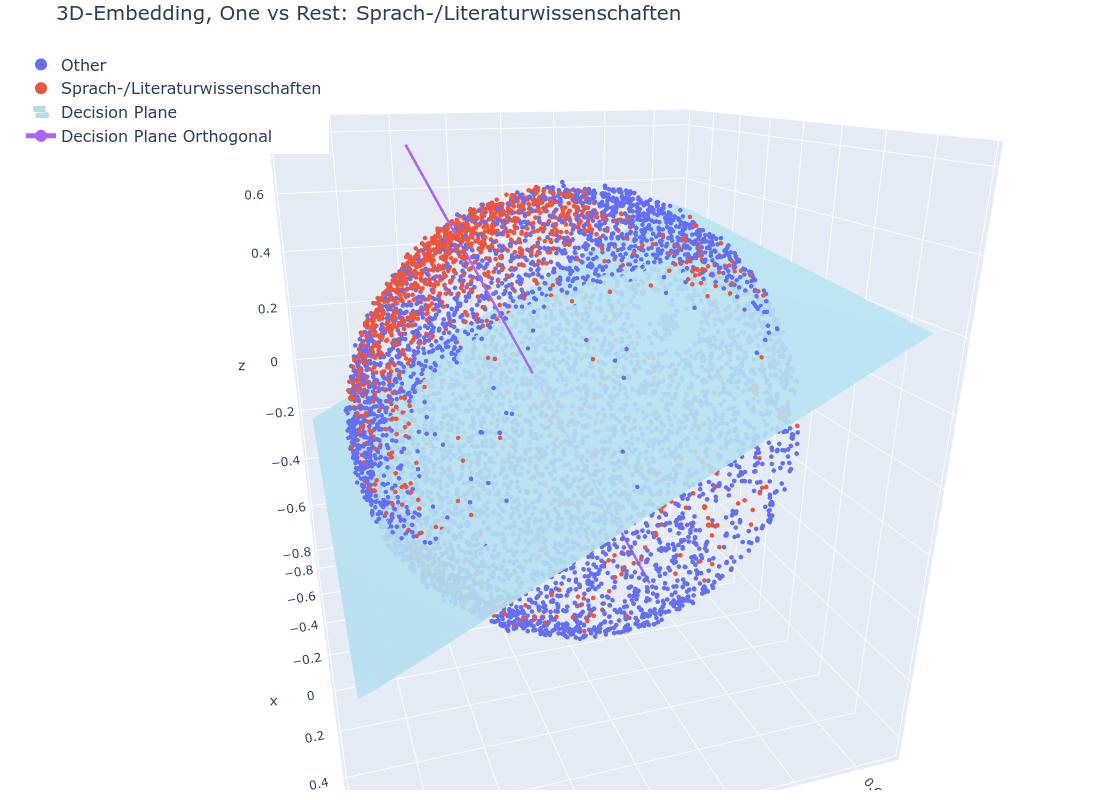
\includegraphics[width=1.1\textwidth]{graphics/dataset_new/possibledecision_sprachlit.png}
		\slcaption{A possible Hyperplane on a 3-Dimensional Embedding. The SVM depicted here would reach an Accuracy of 67.9\% (Precision: 39.8\%, Recall: 70.5\%). Visualize interactively: \url{https://github.com/cstenkamp/derive_conceptualspaces/blob/main/notebooks/text_referenced_plots/visualize_embeddings_mds.ipynb} }
		\label{fig:mds_3d_hyperplane}
		%TODO: why do I have this plot? -> To say what the lower boundary of what a 3D-Embedding of NON-CLASS-SPECIFIC dimensions can yield for classification
	  }
	\end{center}
\end{figure}

\includeMD{pandoc_generated_latex/4_1_qualitativeresults}

\section{Quantiative Analysis}

\todoparagraph{As described in} \autoref{sec:workflow}, a good first approximation is to check how many candidate-terms we get. \autoref{tab:kappa_table} shows the results of many runs with different parameter-combinations with the purpose of figuring out which combination of parameters and kappa-metrics lead to enough candidate-terms (\todoparagraph{Also ref the figure of workflow where I check what threshold was realistic})


\begin{table}[h]
	\resizebox{\textwidth}{!}{%
	\begin{tabular}{llllrrrrrrrrr}
	\toprule
% 	 &  &  &  & \rotatebox{70}{\textbf{k_r2r_d}} & \rotatebox{70}{\textbf{k_r2r_min}} & \rotatebox{70}{\textbf{k_dig}} & \rotatebox{70}{\textbf{k_r2r+_d}} & \rotatebox{70}{\textbf{k_r2r+_min}} & \rotatebox{70}{\textbf{k_r2r+_max}} & \rotatebox{70}{\textbf{k_dig+_2}} & \rotatebox{70}{\textbf{k_c2r+}} & \rotatebox{70}{\textbf{mean}} \\
	\textbf{Preprocessing} & \specialcell[b]{\textbf{Quanti-}\\ \textbf{fication}} & \textbf{\#Dims} & \specialcell[b]{\textbf{Doc-Term-}\\ \textbf{Matrix} \\ \textbf{Quanti-}\\ \textbf{fication}} & \rotatebox{70}{\textbf{k_r2r_d}} & \rotatebox{70}{\textbf{k_r2r_min}} & \rotatebox{70}{\textbf{k_dig}} & \rotatebox{70}{\textbf{k_r2r+_d}} & \rotatebox{70}{\textbf{k_r2r+_min}} & \rotatebox{70}{\textbf{k_r2r+_max}} & \rotatebox{70}{\textbf{k_dig+_2}} & \rotatebox{70}{\textbf{k_c2r+}} & \rotatebox{70}{\textbf{mean}} \\
	\midrule
	\multirow[t]{24}{*}{\mfauhcsdT} & \multirow[t]{8}{*}{\textbf{count}} & \multirow[t]{2}{*}{\textbf{3}} & \textbf{ppmi} & 0 & 1 & 0 & 145 & 370 & 510 & 191 & - & 174 \\
	 &  &  & \textbf{tfidf} & 0 & 1 & 0 & 110 & 237 & 278 & 83 & - & 101 \\
	\cline{3-4}
	 &  & \multirow[t]{3}{*}{\textbf{100}} & \textbf{count} & 0 & 5 & 0 & 0 & 114 & 52 & 290 & 0 & 58 \\
	 &  &  & \textbf{ppmi} & 0 & 6 & 27 & 139 & 224 & 247 & 120 & - & 109 \\
	 &  &  & \textbf{tfidf} & 0 & 6 & 5 & 246 & 270 & 281 & 201 & - & 144 \\
	\cline{3-4}
	 &  & \multirow[t]{3}{*}{\textbf{200}} & \textbf{count} & 0 & 5 & 1 & 0 & 133 & 52 & 509 & 0 & 88 \\
	 &  &  & \textbf{ppmi} & 0 & 6 & 57 & 196 & 315 & 344 & 90 & - & 144 \\
	 &  &  & \textbf{tfidf} & 0 & 6 & 17 & 357 & 370 & 372 & 433 & - & 222 \\
	\cline{2-4} \cline{3-4}
	 & \multirow[t]{8}{*}{\textbf{ppmi}} & \multirow[t]{2}{*}{\textbf{3}} & \textbf{ppmi} & 0 & 0 & 0 & 192 & 247 & 363 & 136 & - & 134 \\
	 &  &  & \textbf{tfidf} & 0 & 0 & 0 & 169 & 206 & 217 & 59 & - & 93 \\
	\cline{3-4}
	 &  & \multirow[t]{3}{*}{\textbf{100}} & \textbf{count} & 0 & 0 & 0 & 0 & 38 & 25 & 242 & 0 & 38 \\
	 &  &  & \textbf{ppmi} & 0 & 0 & 0 & 80 & 112 & 101 & 22 & - & 45 \\
	 &  &  & \textbf{tfidf} & 0 & 0 & 0 & 89 & 90 & 96 & 85 & - & 51 \\
	\cline{3-4}
	 &  & \multirow[t]{3}{*}{\textbf{200}} & \textbf{count} & 0 & 0 & 0 & 0 & 34 & 21 & 293 & 0 & 44 \\
	 &  &  & \textbf{ppmi} & 0 & 1 & 112 & 100 & 163 & 163 & 37 & - & 82 \\
	 &  &  & \textbf{tfidf} & 0 & 1 & {\cellcolor{lightgreen}} 127 & 99 & 107 & 106 & 131 & - & 82 \\
	\cline{2-4} \cline{3-4}
	 & \multirow[t]{8}{*}{\textbf{tfidf}} & \multirow[t]{2}{*}{\textbf{3}} & \textbf{ppmi} & 0 & 0 & 0 & 229 & 357 & 423 & 84 & - & 156 \\
	 &  &  & \textbf{tfidf} & 0 & 0 & 0 & 169 & 255 & 258 & 24 & - & 101 \\
	\cline{3-4}
	 &  & \multirow[t]{3}{*}{\textbf{100}} & \textbf{count} & 0 & 1 & 0 & 0 & 162 & 64 & 450 & 0 & 85 \\
	 &  &  & \textbf{ppmi} & 0 & 1 & 3 & 324 & 404 & 423 & 151 & - & 187 \\
	 &  &  & \textbf{tfidf} & 0 & 1 & 0 & 390 & 422 & 437 & 425 & - & 239 \\
	\cline{3-4}
	 &  & \multirow[t]{3}{*}{\textbf{200}} & \textbf{count} & 0 & 2 & 0 & 0 & 211 & 83 & {\cellcolor{lightgreen}} 869 & {\cellcolor{lightgreen}} 1 & 146 \\
	 &  &  & \textbf{ppmi} & 0 & 2 & 13 & 395 & {\cellcolor{lightgreen}} 559 & {\cellcolor{lightgreen}} 577 & 153 & - & 243 \\
	 &  &  & \textbf{tfidf} & 0 & 2 & 0 & {\cellcolor{lightgreen}} 531 & 554 & 572 & 794 & - & {\cellcolor{lightgreen}} 350 \\
	\cline{1-4} \cline{2-4} \cline{3-4}
	\multirow[t]{24}{*}{\mfauhtcsldp} & \multirow[t]{8}{*}{\textbf{count}} & \multirow[t]{2}{*}{\textbf{3}} & \textbf{ppmi} & 0 & 1 & 0 & 226 & 319 & 317 & 208 & - & 153 \\
	 &  &  & \textbf{tfidf} & 0 & 1 & 0 & 210 & 214 & 215 & 82 & - & 103 \\
	\cline{3-4}
	 &  & \multirow[t]{3}{*}{\textbf{100}} & \textbf{count} & 0 & 7 & 0 & 0 & 118 & 61 & 230 & 0 & 52 \\
	 &  &  & \textbf{ppmi} & 0 & 8 & 27 & 184 & 256 & 262 & 125 & - & 123 \\
	 &  &  & \textbf{tfidf} & 0 & 8 & 5 & 253 & 255 & 255 & 168 & - & 135 \\
	\cline{3-4}
	 &  & \multirow[t]{3}{*}{\textbf{200}} & \textbf{count} & 0 & 8 & 0 & 0 & 117 & 64 & 290 & 0 & 60 \\
	 &  &  & \textbf{ppmi} & 0 & {\cellcolor{lightgreen}} 11 & 41 & 200 & 319 & 325 & 88 & - & 141 \\
	 &  &  & \textbf{tfidf} & 0 & {\cellcolor{lightgreen}} 11 & 8 & 331 & 333 & 333 & 302 & - & 188 \\
	\cline{2-4} \cline{3-4}
	 & \multirow[t]{8}{*}{\textbf{ppmi}} & \multirow[t]{2}{*}{\textbf{3}} & \textbf{ppmi} & 0 & 0 & 0 & 138 & 310 & 321 & 254 & - & 146 \\
	 &  &  & \textbf{tfidf} & 0 & 0 & 0 & 143 & 148 & 150 & 187 & - & 90 \\
	\cline{3-4}
	 &  & \multirow[t]{3}{*}{\textbf{100}} & \textbf{count} & 0 & 0 & 0 & 0 & 29 & 11 & 186 & 0 & 28 \\
	 &  &  & \textbf{ppmi} & 0 & 1 & 0 & 117 & 142 & 142 & 20 & - & 60 \\
	 &  &  & \textbf{tfidf} & 0 & 1 & 0 & 122 & 124 & 124 & 103 & - & 68 \\
	\cline{3-4}
	 &  & \multirow[t]{3}{*}{\textbf{200}} & \textbf{count} & 0 & 1 & 0 & 0 & 25 & 10 & 272 & 0 & 38 \\
	 &  &  & \textbf{ppmi} & 0 & 1 & 48 & 126 & 161 & 165 & 28 & - & 76 \\
	 &  &  & \textbf{tfidf} & 0 & 1 & 17 & 143 & 144 & 148 & 133 & - & 84 \\
	\cline{2-4} \cline{3-4}
	 & \multirow[t]{8}{*}{\textbf{tfidf}} & \multirow[t]{2}{*}{\textbf{3}} & \textbf{ppmi} & 0 & 0 & 0 & 146 & 219 & 223 & 133 & - & 103 \\
	 &  &  & \textbf{tfidf} & 0 & 0 & 0 & 108 & 111 & 109 & 38 & - & 52 \\
	\cline{3-4}
	 &  & \multirow[t]{3}{*}{\textbf{100}} & \textbf{count} & 0 & 1 & 0 & 0 & 160 & 54 & 389 & 0 & 76 \\
	 &  &  & \textbf{ppmi} & 0 & 2 & 9 & 281 & 375 & 380 & 205 & - & 179 \\
	 &  &  & \textbf{tfidf} & 0 & 2 & 0 & 373 & 377 & 392 & 339 & - & 212 \\
	\cline{3-4}
	 &  & \multirow[t]{3}{*}{\textbf{200}} & \textbf{count} & 0 & 3 & 0 & 0 & 199 & 64 & 661 & 0 & 116 \\
	 &  &  & \textbf{ppmi} & 0 & 3 & 21 & 362 & 456 & 472 & 164 & - & 211 \\
	 &  &  & \textbf{tfidf} & 0 & 3 & 1 & 499 & 498 & 501 & 645 & - & 307 \\
	\bottomrule
	\end{tabular}
	}
	\caption{Number of Candidate-Phrases for different parameter-combinations and kappa-values \label{tab:kappa_table}}
	\label{tab:cands_per_config}
\end{table}


\includeMD{pandoc_generated_latex/4_2_quantitativeresults}

\section{Conclusion for Results}

\includeMD{pandoc_generated_latex/4_3_resultsconclusion}